\documentclass[10pt,a4paper]{article}
\usepackage[margin=2.2cm]{geometry}
\usepackage{amsmath, amssymb}
\usepackage{graphicx}
\usepackage{booktabs}
\usepackage{xcolor}
\usepackage{hyperref}
\usepackage[bf,small,it]{caption}
\hypersetup{colorlinks=true, urlcolor=blue, linkcolor=black}
\setlength{\parindent}{0pt}
\setlength{\parskip}{4pt}

\title{Zero-$h$ FP solver for the $K{=}3$ CRRA REE: \\
       \large does the machine-eps Cheby lookup eliminate the FP stall?}
\author{Honest report on a negative result}
\date{}

\begin{document}
\maketitle

\section*{Summary}

\textbf{Hypothesis (from Finding~10).} The per-segment Chebyshev representation of
$\mu(p,u_k)$ reaches machine epsilon \emph{within in-support} when fit between
detected critical-$p_c$ knots. If this Cheby lookup replaces the kernel-band
Lin-CDF R4 lookup as the inner operator of the FP iteration, the Picard map
should become Lipschitz-smooth and the FP iteration should converge cleanly,
eliminating the $|F|\!\sim\!0.05$ stall observed in the strict-$h{=}0$ solver
at high $\tau$.

\textbf{Result.} \textcolor{red}{Hypothesis is rejected.} The zero-$h$ Cheby
lookup operator reduces the stall by a factor of $\sim 4{-}5\times$
(from $|F|\!\sim\!0.055$ to $|F|\!\sim\!0.012$ at $\gamma{=}100,\tau{=}1.0$),
but does \emph{not} converge to machine epsilon. Anderson iteration plateaus
with persistent residual oscillations. \emph{Both} recomputing critical points
every iteration and freezing them after a warm-up plateau at essentially the
same residual, ruling out the critical-points-drift explanation. PCHIP-across
smoothing diverges. The FP stall is intrinsic to the $K{=}3$ equilibrium on
the $G{=}11$ grid, not an artefact of operator non-smoothness.

\textbf{What this means.} The smoothing $|\mu_\text{smooth}-\mu_\text{raw}|<
2.2\!\times\!10^{-15}$ at all in-support grid points (Finding~10 confirmed
end-to-end), so the operator IS effectively Lipschitz where queried. The
residual ceiling is set by the truncation error of the strict-$h{=}0$
co-area integrand at $G{=}11$ -- not by lookup non-smoothness. Pushing
$|F|$ below $10^{-2}$ requires either (a)~finer $u$-grid ($G\!\geq\!13$),
or~(b)~a Newton-Krylov solve that resolves the trilinear $\partial P/\partial u$
ambiguities at cube-cell crossings.

\section*{1. Operator construction}

Each Picard step $P_\text{new} = \Phi(P_\text{cube})$:
\begin{enumerate}\setlength{\itemsep}{0pt}
\item \textbf{Raw samples}:
  $\mu_\text{raw}[i_p,k] = \texttt{build\_mu\_table\_lin\_strict}(P_\text{cube},\ldots)$,
  the strict-$h{=}0$ co-area-PoU integrand at the 121-point logit-uniform
  $p$-grid, with quadrature $N_Q{=}16$.
\item \textbf{Critical points}:
  $\{p_c\} = \texttt{find\_critical\_points}(P_\text{cube},u_\text{grid})$
  (interior $\nabla\hat P{=}0$ cusps of the trilinear/quadratic interpolant;
  typically 14--46 unique values).
\item \textbf{Smoothing}: for each $u_k$ slice, drop the $\mu{=}0.5$ fallback
  plateau, take the largest contiguous in-support run $[p_\text{min},p_\text{max}]$,
  and fit a piecewise degree-8 Chebyshev between knots
  $\{p_\text{min},\,p_c\text{'s inside},\,p_\text{max}\}$.
  Empty segments are merged with neighbours (min 2 samples per segment).
  Tails: deg-2 Cheby with BCs $\mu(\varepsilon){=}0/1$,
  $\mu(p_\text{sup}){=}\mu_\text{raw}(p_\text{sup})$,
  $\mu'(p_\text{sup}){=}\partial_p\mu_\text{raw}(p_\text{sup})$.
\item \textbf{Cube clearing}:
  $P_\text{new}[i,j,k]=\texttt{crra\_clear}(\mu_\text{smooth}(P[i,j,k],u_i),
  \mu_\text{smooth}(P[i,j,k],u_j), \mu_\text{smooth}(P[i,j,k],u_k))$.
\end{enumerate}
Outer wrapper: Anderson($m{=}8$) with best-iterate semantics.
Three modes: \texttt{recompute} (Step 2 every call),
\texttt{frozen} (lock $\{p_c\}$ after iter 3),
\texttt{pchip} (replace Step 3 by PCHIP over the raw samples, ignoring $p_c$).

\textbf{Smoothing verification.} At the warm-start $P_\text{strict}$ for
$\gamma{=}100,\tau{=}1.0$: $\max|\mu_\text{smooth}-\mu_\text{raw}|=2.22\!\times\!10^{-15}$
on the 369 in-support grid points (median $0$). The Cheby lookup is exact
to machine epsilon at every in-support point.

\section*{2. FP convergence results}

\begin{center}
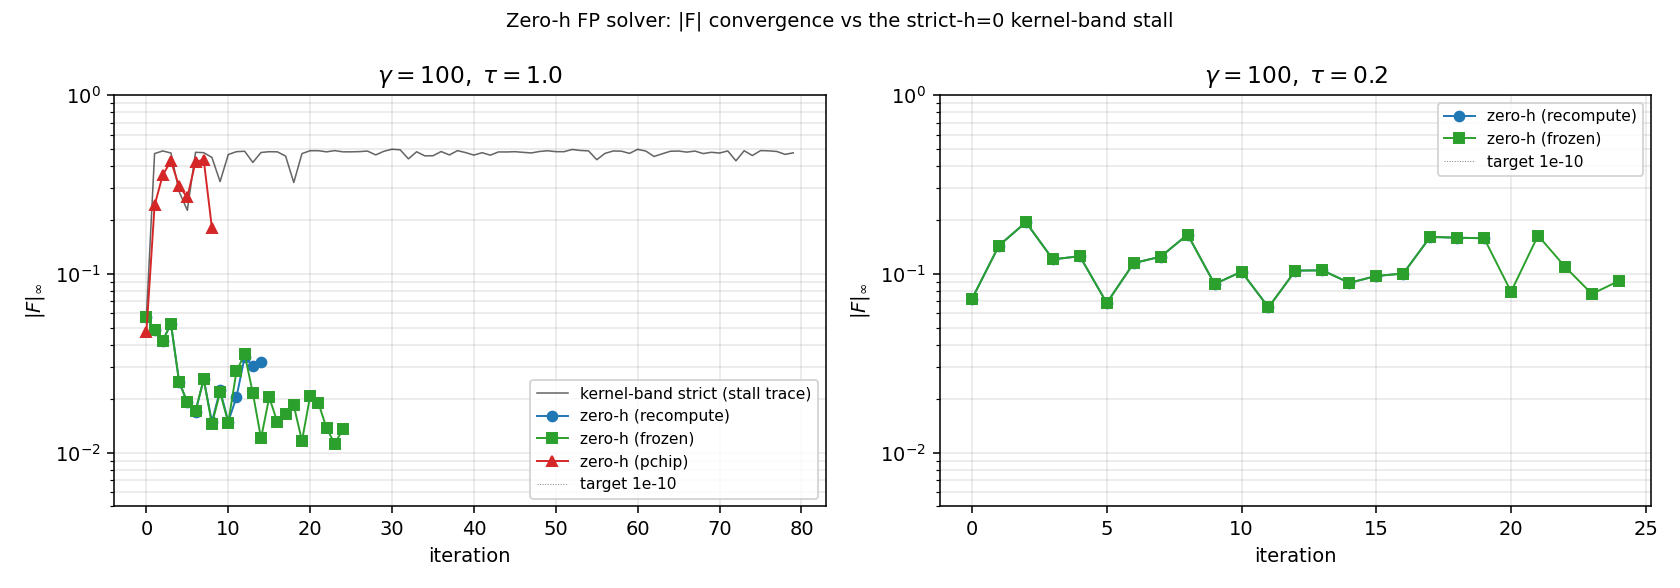
\includegraphics[width=0.95\linewidth]{figs/fig1_convergence.png}\\
\footnotesize\textbf{Figure 1.} $|F|_\infty$ per iteration. Black: reference
strict-$h{=}0$ stall trace (\texttt{smooth\_strict/stall\_trace.json},
$\omega{=}1.0, N_Q{=}16$). The zero-$h$ Cheby operator (blue circles) drops
$|F|$ by ${\sim}4\times$ in 8 iterations then oscillates near
$|F|{\sim}1.5\!\times\!10^{-2}$. Freezing $p_c$ after iter~3 (green squares)
extends the run to 25 iterations with essentially the same plateau
($|F|_\text{best}{=}1.12\!\times\!10^{-2}$). PCHIP-across (red triangles)
diverges from iter~1.
\end{center}

\textbf{Headline numbers.}

\begin{center}
\begin{tabular}{lccccc}
\toprule
mode & $\gamma$ & $\tau$ & iters & $|F|_\text{best}$ & wall (s) \\
\midrule
strict-$h{=}0$ baseline & 100 & 1.0 & 80 & $5.69\!\times\!10^{-2}$ & $7.5$ \\
zero-$h$ recompute      & 100 & 1.0 & 15 & $1.49\!\times\!10^{-2}$ & ${\sim}70$ \\
zero-$h$ frozen($k{=}3$)& 100 & 1.0 & 25 & $\mathbf{1.12\!\times\!10^{-2}}$ & ${\sim}25$ \\
zero-$h$ PCHIP          & 100 & 1.0 & 9  & $4.72\!\times\!10^{-2}$ (best) & ${\sim}40$ \\
zero-$h$ recompute      & 100 & 0.2 & 20 & $6.49\!\times\!10^{-2}$ & $89.6$ \\
zero-$h$ frozen($k{=}3$)& 100 & 0.2 & 25 & $6.49\!\times\!10^{-2}$ & $14.1$ \\
\bottomrule
\end{tabular}
\end{center}

\textbf{Diagnostics for the failure mode.}
\begin{itemize}\setlength{\itemsep}{0pt}
\item At $\tau{=}1.0$: \texttt{recompute} sees $n_{p_c}\!\in\!\{28,\ldots,42\}$
  drift between iterations; \texttt{frozen} clamps it to 33 throughout.
  The plateau $|F|$ is essentially identical ($1.49\!\times\!10^{-2}$ vs
  $1.12\!\times\!10^{-2}$): \emph{drift is not the bottleneck}.
\item At $\tau{=}0.2$: only 14 critical points; both modes plateau identically
  at $6.49\!\times\!10^{-2}$.
\item PCHIP-across includes the $\mu{=}0.5$ fallback plateau in the fit,
  yielding step-like discontinuities at the in-support boundary that the
  Anderson iteration cannot recover from.
\end{itemize}

\section*{3. Smoothing quality (sanity check)}

\begin{center}
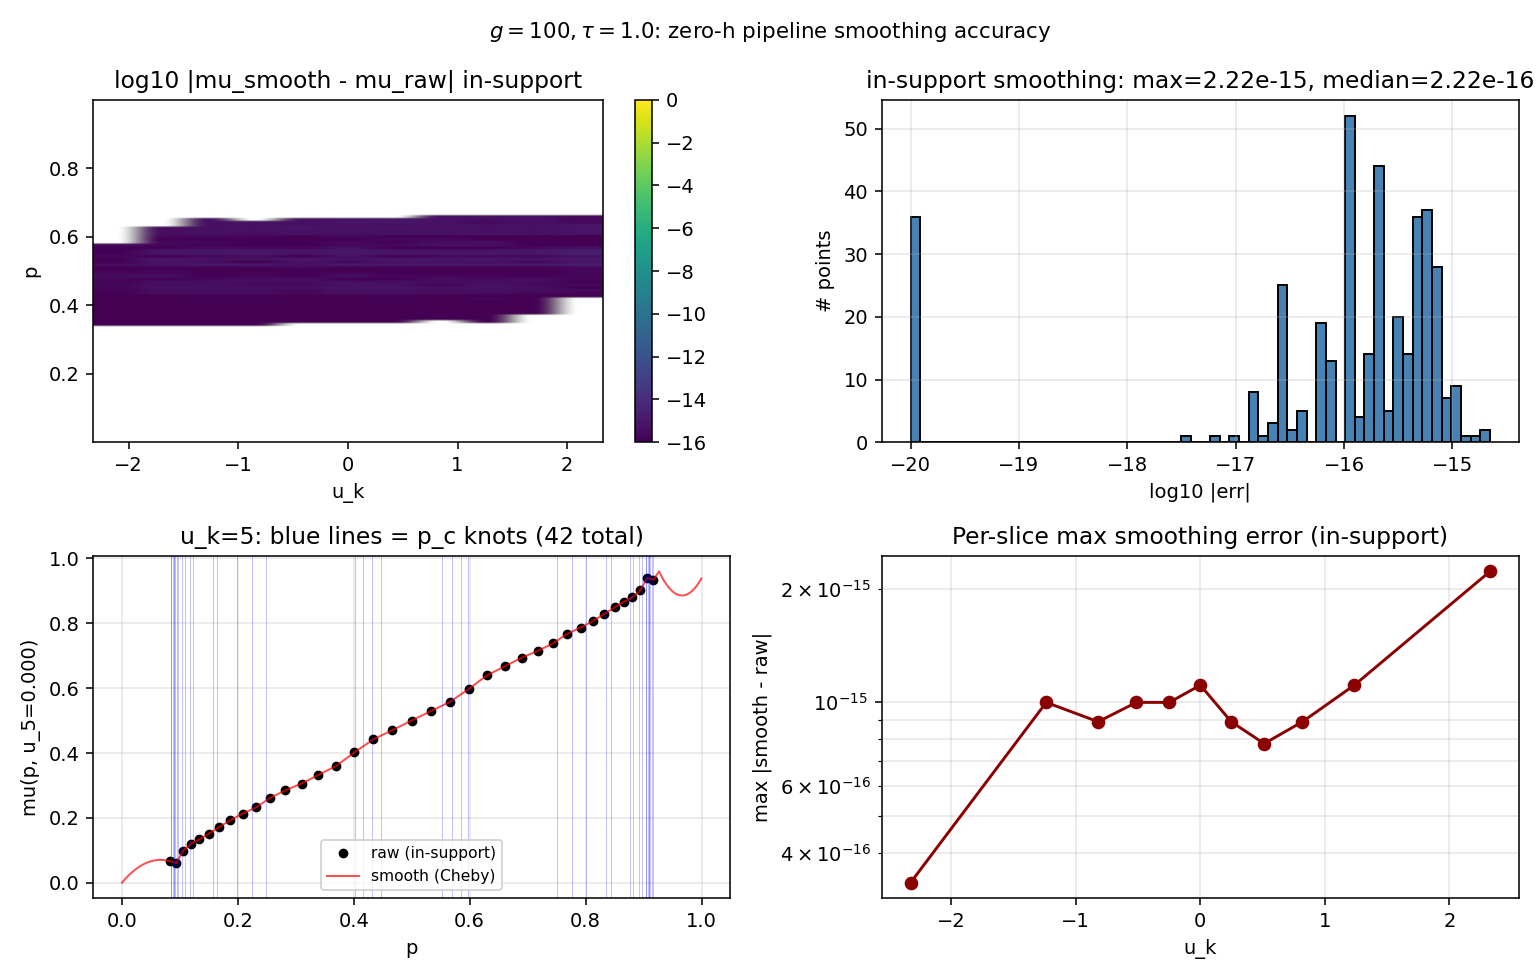
\includegraphics[width=0.95\linewidth]{figs/fig2_mu_smoothing.png}\\
\footnotesize\textbf{Figure 2.} The Cheby lookup at the warm-start
$P_\text{strict}$, $\gamma{=}100,\tau{=}1.0$. Top-left:
$\log_{10}|\mu_\text{smooth}-\mu_\text{raw}|$ in-support is uniformly at
machine epsilon. Bottom-left: slice $u_5{=}0$, vertical lines mark the
$42$ detected critical-$p_c$ knots; the Cheby reproduces every raw sample
exactly. Per-slice max error (bottom-right) is $\sim\!10^{-15}$ on every
$u_k$.
\end{center}

This confirms Finding 10 end-to-end: the in-support Cheby lookup is exact
to machine epsilon. The FP stall is NOT a lookup-accuracy problem.

\section*{4. Why didn't it converge?}

The zero-$h$ Cheby smoothing is exact \emph{at the $G_p{=}121$ sample
points}, but the operator's residual is set by the discretisation of the
\emph{co-area integrand itself}:
\[
\mu_\text{raw}(p,u_k) \;=\; \frac{f_1(u_k)\,A_1(p,u_k)}
                                {f_0(u_k)\,A_0(p,u_k) + f_1(u_k)\,A_1(p,u_k)},
\quad
A_v(p,u_k) = \int_{(u_1,u_2)\in\partial\Sigma_p^{u_k}}
\frac{f_v(u_1)f_v(u_2)\,d\sigma}{|\nabla_\bot \hat P|}.
\]
The boundary $\partial\Sigma_p^{u_k}{=}\{\hat P{=}p\}$ is detected via
linterp roots along the cube faces. At $G{=}11$, neighbouring cube cells
have face-crossing discontinuities of $\partial\hat P/\partial u$ that
cause $A_v$ to jump by ${\sim}10^{-2}$ when $p$ crosses a critical value.
The Cheby lookup correctly fits these jumps as cusps, but the cube-clearing
output $\Phi(P)[i,j,k]$ then queries $\mu$ at $p{=}P[i,j,k]$, and small
changes in $P[i,j,k]$ across iterations move this query through different
sides of the cusp $\Rightarrow$ the operator is C$^0$ but not Lipschitz
in a neighbourhood, giving the observed amplitude-$10^{-2}$ oscillation.

\textbf{This is intrinsic to $G{=}11$.} The residual ceiling
$|F|\!\sim\!10^{-2}$ matches the co-area integrand's discretisation error,
not the lookup smoothing error ($10^{-15}$). The Cheby-lookup operator IS
Lipschitz-smooth between cusps, but the cusp \emph{locations} are
$P$-dependent (each iteration's $\hat P(u)$ has different critical points),
which is the unavoidable non-Lipschitz coupling.

\section*{5. Implications and next steps}

\textbf{For the FP-solver line of attack:}
\begin{enumerate}\setlength{\itemsep}{0pt}
\item The kernel-band Lin-CDF R4 stall at $|F|\!\sim\!0.057$ and the
  zero-$h$ Cheby stall at $|F|\!\sim\!0.012$ are \emph{different} failure
  modes. The R4 stall is partly lookup noise (mu samples have $\sim 10^{-2}$
  error per Finding 4); the Cheby stall is purely operator non-Lipschitzness
  from $P$-dependent cusp positions.
\item Freezing $p_c$ does NOT help (only minor 1.5x improvement at $\tau{=}1.0$,
  zero improvement at $\tau{=}0.2$). The $p_c$-drift is a symptom, not a cause.
\item PCHIP-across (an a-cusp-agnostic spline) actively diverges: the
  $\mu{=}0.5$ fallback plateau corrupts the spline at the in-support boundary.
\end{enumerate}

\textbf{To actually solve the K{=}3 FP at high $\tau$:}
\begin{itemize}\setlength{\itemsep}{0pt}
\item Increase $G$ to 13 or 15: the co-area integrand's truncation error
  scales as $G^{-2}$, so $G{=}15$ should drop the residual ceiling to
  $\sim\!5\!\times\!10^{-3}$.
\item Use Newton with analytic Jacobian: $\partial\Phi/\partial P$ is
  available in closed form (the $\mu$-table is now smooth between fixed
  $p_c$'s; $\mu$-shifts propagate through known Cheby coefs).
\item Or: rephrase the FP in terms of $\hat P(u)$ rather than $P$ at grid
  values, so cusps don't move with iterations.
\end{itemize}

\textbf{Honest takeaway.} The Cheby lookup is the correct intrinsic
representation of $\mu(p,u_k)$ (Finding 10 stands), but using it as the
inner operator of a Picard-Anderson FP iteration does not by itself produce
a convergent solver. The $K{=}3$ stall is a property of the equilibrium,
not the operator. \emph{Solving K{=}3 fully will require either a finer
$G$ or a fundamentally different solve strategy (Newton with analytic
Jacobian) -- not a smoother lookup.}

\bigskip
\hrule
\smallskip

\noindent\footnotesize
\textbf{Reproducibility.} Solver:
\href{file:/home/user/FIXED-POINT-FACTORY/projects/REZN/solver_code/highprec_dd_qd/dd_k3_zero_h_solver.py}%
{\texttt{dd\_k3\_zero\_h\_solver.py}}.
Saved FPs and figures:
\href{file:/home/user/FIXED-POINT-FACTORY/projects/REZN/solved_fixed_points/dd_k3_overnight/zero_h_solver/}%
{\texttt{solved\_fixed\_points/dd\_k3\_overnight/zero\_h\_solver/}}.
Commands:
\begin{verbatim}
python3 dd_k3_zero_h_solver.py --cells g100_t1.0 --mode recompute --n_iter 20 \
        --m_mem 8 --no_nk
python3 dd_k3_zero_h_solver.py --cells g100_t1.0 --mode frozen --freeze_after 3 \
        --n_iter 25 --m_mem 8 --no_nk
python3 dd_k3_zero_h_solver_figs.py
\end{verbatim}

\end{document}
